%\documentclass[hyperref={pdfpagelabels=false},slidetop,9pt]{beamer}
\documentclass[slidetop,8pt]{beamer}
\usepackage[T1]{fontenc}
\usepackage[utf8]{inputenc}
\newcommand{\id}{30}
\newcommand{\nom}{Calculs d'hyperstatisme}
\newcommand{\sequence}{04}
\newcommand{\nomsequence}{Liaisons entre les solides}
\newcommand{\num}{03}
\newcommand{\type}{TD}
\newcommand{\descrip}{En appliquant les règles de la théorie des mécanisme, déterminer le degré d'hyperstatisme de plusieurs systèmes et proposer des solutions afin de diminuer ce degré}
\newcommand{\competences}{B2-12: Proposer une modélisation des liaisons avec leurs caractéristiques géométriques. \\ &  B2-13: Proposer un modèle cinématique paramétré à partir d'un système réel, d'une maquette numérique ou d'u \\ &  B2-17: Simplifier un modèle de mécanisme. \\ &  B2-18: Modifier un modèle pour le rendre isostatique.}
\newcommand{\nbcomp}{4}
\newcommand{\systemes}{E.P.A.S, Machine d'essai de traction}
\newcommand{\systemesnum}{14, 13}
\newcommand{\systemessansaccent}{E.P.A.S, Machine d'essai de traction}
\newcommand{\ilot}{3}
\newcommand{\ilotstr}{03}
\newcommand{\dossierilot}{\detokenize{Ilot_03 E.P.A.S, Machine d'essai de traction}}
\newcommand{\imageun}{EPAS}
\newcommand{\imagedeux}{Machine_dessai_de_traction}

\usepackage{etex}
\usepackage{tikz}
\usepackage[european]{circuitikz}
\usepackage{pgf}
\usepackage[all]{xy}
\usepackage{pgfpages}
\usepackage{graphbox}
\usepackage{pdfpages}
%\usepackage[adobe-utopia]{mathdesign}
\usepackage{ifthen}
\usepackage{cancel}
\usepackage{framed}
\usepackage{subfig}
\usepackage{tabularx}
\usepackage{setspace}
\usepackage{soul}
\usepackage{schemabloc}
\usepackage{eqnarray}
\usepackage[dot, phantomtext]{dashundergaps}
\usepackage{media9}
\usepackage{multimedia}
\usepackage{textcomp}
\usefonttheme[onlymath]{serif}

\author{Renaud Costadoat}
\institute{Lycée Dorian}

\usepackage{multido}
\usepackage{multirow}
\usepackage{multicol} % Portions de texte en colonnes
\usepackage{flafter}%floatants après la référence

\usepackage{color}
\usepackage{xcolor}
\usepackage{colortbl}

\usepackage[gen]{eurosym}
\usepackage{tikz}
%\usepackage{pstricks,pst-node,pst-tree,pst-solides3d}
\usepackage{lmodern}
\usepackage[francais]{babel}
\usepackage{pslatex}
\usetheme{renaud}
\usepackage{times}
\usepackage[frenchmath]{newtxsf} % for sans serif symbols
\renewcommand{\familydefault}{\sfdefault}
%\usepackage{amsfonts}
%\usepackage{amsmath}
%\usepackage{mathastext}
\usepackage{verbatim}
\usepackage{moreverb}
%\usetikzlibrary{arrows,shapes}
\usepackage{graphicx}
\usepackage{psfrag}
\usepackage{wrapfig}
\usepackage{etoolbox}

\definecolor{gris25}{gray}{0.75}
\definecolor{bleu}{RGB}{18,33,98}
\definecolor{bleuf}{RGB}{42,94,171}
\definecolor{bleuc}{RGB}{231,239,247}
\definecolor{rougef}{RGB}{185,18,27}
\definecolor{rougec}{RGB}{255,188,204}%255,230,231
\definecolor{vertf}{RGB}{103,126,82}
\definecolor{vertc}{RGB}{220,255,191}

\setlength\parindent{24pt}
\parskip 7.2pt
\parindent 8pt

\newenvironment{rem}[1][\hsize]%
{%
    \def\FrameCommand
   {%
\rotatebox{90}{\textit{\textsf{Remarque}}} 
       {\color{bleuf}\vrule width 3pt}%
       \hspace{0pt}%must no space.
       \fboxsep=\FrameSep\colorbox{bleuc}%
  }%
    \MakeFramed{\hsize#1\advance\hsize-\width\FrameRestore}%
}%
{\endMakeFramed}%


\newenvironment{savoir}[1][\hsize]%
{%
    \def\FrameCommand
    {%
\rotatebox{90}{\textit{\textsf{Savoir}}} 
        {\color{bleuf}\vrule width 3pt}%
        \hspace{0pt}%must no space.
        \fboxsep=\FrameSep\colorbox{bleuc}%
    }%
    \MakeFramed{\hsize#1\advance\hsize-\width\FrameRestore}%
}%
{\endMakeFramed}%

\newenvironment{prob}[1][\hsize]%
{%
    \def\FrameCommand%
    {%
\rotatebox{90}{\textit{\textsf{Problematique}}} 
        {\color{rougef}\vrule width 3pt}%
        \hspace{0pt}%must no space.
        \fboxsep=\FrameSep\colorbox{rougec}%
    }%
    \MakeFramed{\hsize#1\advance\hsize-\width\FrameRestore}%
}%
{\endMakeFramed}%

\newenvironment{obj}[1][\hsize]%
{%
    \def\FrameCommand%
    {%
\rotatebox{90}{\textit{\textsf{Objectif}}} 
        {\color{vertf}\vrule width 3pt}%
        \hspace{0pt}%must no space.
        \fboxsep=\FrameSep\colorbox{vertc}%
    }%
    \MakeFramed{\hsize#1\advance\hsize-\width\FrameRestore}%
}%
{\endMakeFramed}%

\newenvironment{defi}[1][\hsize]%
{%
    \def\FrameCommand%
    {%
\rotatebox{90}{\textit{\textsf{Definition}}} 
        {\color{bleuf}\vrule width 3pt}%
        \hspace{0pt}%must no space.
        \fboxsep=\FrameSep\colorbox{rougec}%
    }%
    \MakeFramed{\hsize#1\advance\hsize-\width\FrameRestore}%
}%
{\endMakeFramed}%


\newenvironment{hypo}[1][\hsize]%
{%
    \def\FrameCommand%
    {%
\rotatebox{90}{\textit{\textsf{Hypothèse\\}}} 
        {\color{bleuf}\vrule width 3pt}%
        \hspace{0pt}%must no space.
        \fboxsep=\FrameSep\colorbox{bleuc}%
    }%
    \MakeFramed{\hsize#1\advance\hsize-\width\FrameRestore}%
}%
{\endMakeFramed}%


\newenvironment{prop}[1][\hsize]%
{%
    \def\FrameCommand%
    {%
\rotatebox{90}{\textit{\textsf{Propriété}}} 
        {\color{bleuf}\vrule width 3pt}%
        \hspace{0pt}%must no space.
        \fboxsep=\FrameSep\colorbox{bleuc}%
    }%
    \MakeFramed{\hsize#1\advance\hsize-\width\FrameRestore}%
}%
{\endMakeFramed}%

\newenvironment{props}[1][\hsize]%
{%
    \def\FrameCommand%
    {%
\rotatebox{90}{\textit{\textsf{Propriétés}}} 
        {\color{bleuf}\vrule width 3pt}%
        \hspace{0pt}%must no space.
        \fboxsep=\FrameSep\colorbox{bleuc}%
    }%
    \MakeFramed{\hsize#1\advance\hsize-\width\FrameRestore}%
}%
{\endMakeFramed}%

\newenvironment{exemple}[1][\hsize]%
{%
    \def\FrameCommand%
    {%
\rotatebox{90}{\textit{\textsf{Exemple}}} 
        {\color{vertf}\vrule width 3pt}%
        \hspace{0pt}%must no space.
        \fboxsep=\FrameSep\colorbox{vertc}%
    }%
    \MakeFramed{\hsize#1\advance\hsize-\width\FrameRestore}%
}%
{\endMakeFramed}%

\newenvironment{resultat}[1][\hsize]%
{%
    \def\FrameCommand%
    {%
\rotatebox{90}{\textit{\textsf{Résultat}}} 
        {\color{rougef}\vrule width 3pt}%
%        {\color{bleuf}\vrule width 3pt}%
        \hspace{0pt}%must no space.
        \fboxsep=\FrameSep\colorbox{rougec}%
    }%
    \MakeFramed{\hsize#1\advance\hsize-\width\FrameRestore}%
}%
{\endMakeFramed}%

\newenvironment{methode}[1][\hsize]%
{%
    \def\FrameCommand%
    {%
\rotatebox{90}{\textit{\textsf{Méthode\\}}} 
        {\color{rougef}\vrule width 3pt}%
        \hspace{0pt}%must no space.
        \fboxsep=\FrameSep\colorbox{rougec}%
    }%
    \MakeFramed{\hsize#1\advance\hsize-\width\FrameRestore}%
}%
{\endMakeFramed}%

\newenvironment{theo}[1][\hsize]%
{%
    \def\FrameCommand%
    {%
\rotatebox{90}{\textit{\textsf{Théorème\\}}} 
        {\color{rougef}\vrule width 3pt}%
        \hspace{0pt}%must no space.
        \fboxsep=\FrameSep\colorbox{rougec}%
    }%
    \MakeFramed{\hsize#1\advance\hsize-\width\FrameRestore}%
}%
{\endMakeFramed}%

\newenvironment{warn}[1][\hsize]%
{%
    \def\FrameCommand%
    {%
\rotatebox{90}{\textit{\textsf{Attention\\}}} 
        {\color{rougef}\vrule width 3pt}%
        \hspace{0pt}%must no space.
        \fboxsep=\FrameSep\colorbox{rougec}%
    }%
    \MakeFramed{\hsize#1\advance\hsize-\width\FrameRestore}%
}%
{\endMakeFramed}%

% \usepackage{pstricks}
%\usepackage{minitoc}
% \setcounter{minitocdepth}{4}

\setcounter{tocdepth}{2}

% \mtcselectlanguage{french} 

%\usepackage{draftcopy}% "Brouillon"
% \usepackage{floatflt}
\usepackage{psfrag}
%\usepackage{listings} % Permet d'insérer du code de programmation
\renewcommand{\baselinestretch}{1.2}

% Changer la num�rotation des figures :
% ------------------------------------
% \makeatletter
% \renewcommand{\thefigure}{\ifnum \c@section>\z@ \thesection.\fi
%  \@arabic\c@figure}
% \@addtoreset{figure}{section}
% \makeatother
 


%%%%%%%%%%%%
% Définition des vecteurs %
%%%%%%%%%%%%
 \newcommand{\vect}[1]{\overrightarrow{#1}}

%%%%%%%%%%%%
% Définition des torseusr %
%%%%%%%%%%%%

 \newcommand{\torseur}[1]{%
\left\{{#1}\right\}
}

\newcommand{\torseurcin}[3]{%
\left\{\mathcal{#1} \left(#2/#3 \right) \right\}
}

\newcommand{\torseurstat}[3]{%
\left\{\mathcal{#1} \left(#2\rightarrow #3 \right) \right\}
}

 \newcommand{\torseurc}[8]{%
%\left\{#1 \right\}=
\left\{
{#1}
\right\}
 = 
\left\{%
\begin{array}{cc}%
{#2} & {#5}\\%
{#3} & {#6}\\%
{#4} & {#7}\\%
\end{array}%
\right\}_{#8}%
}

 \newcommand{\torseurcol}[7]{
\left\{%
\begin{array}{cc}%
{#1} & {#4}\\%
{#2} & {#5}\\%
{#3} & {#6}\\%
\end{array}%
\right\}_{#7}%
}

 \newcommand{\torseurl}[3]{%
%\left\{\mathcal{#1}\right\}_{#2}=%
\left\{%
\begin{array}{l}%
{#1} \\%
{#2} %
\end{array}%
\right\}_{#3}%
}

 \newcommand{\vectv}[3]{%
\vect{V\left( {#1} \in {#2}/{#3}\right)}
}


\newcommand{\vectf}[2]{%
\vect{R\left( {#1} \rightarrow {#2}\right)}
}

\newcommand{\vectm}[3]{%
\vect{\mathcal{M}\left( {#1}, {#2} \rightarrow {#3}\right)}
}


 \newcommand{\vectg}[3]{%
\vect{\Gamma \left( {#1} \in {#2}/{#3}\right)}
}

 \newcommand{\vecto}[2]{%
\vect{\Omega\left( {#1}/{#2}\right)}
}

\newcommand{\reponse}[1][4]
{
\multido{}{#1}
{
\begin{center}
\makebox[0.9\linewidth]{\dotfill} \end{center}
}}


% }$$\left\{\mathcal{#1} \right\}_{#2} =%
% \left\{%
% \begin{array}{c}%
%  #3 \\%
%  #4 %
% \end{array}%
% \right\}_{#5}}


%  ------------------------------------------
% | Modification du formatage des sections : | 
%  ------------------------------------------

% Grands titres :
% ---------------

\newcommand{\titre}[1]{%
\begin{center}
      \bigskip
      \rule{\textwidth}{1pt}
      \par\vspace{0.1cm}
      
      \textbf{\large #1}
      \par\rule{\textwidth}{1pt}
    \end{center}
    \bigskip
  }

% Supprime le numéro du chapitre dans la numérotation des sections:
% -----------------------------------------------------------------
\makeatletter
\renewcommand{\thesection}{\@arabic\c@section}
\makeatother


% \titleformat{\chapter}[display]
% {\normalfont\Large\filcenter}
% {}
% {1pc}
% {\titlerule[1pt]
%   \vspace{1pc}%
%   \Huge}[\vspace{1ex}%
% \titlerule]


%%%% Chapitres Comme PY Pechard %%%%%%%%%
% numéro du chapitre
\DeclareFixedFont{\chapnumfont}{OT1}{phv}{b}{n}{80pt}
% pour le mot " Chapitre "
\DeclareFixedFont{\chapchapfont}{OT1}{phv}{m}{it}{40pt}
% pour le titre
\DeclareFixedFont{\chaptitfont}{T1}{phv}{b}{n}{25pt}

\definecolor{gris}{gray}{0.75}
\setbeamertemplate{section in toc}[sections numbered]

\newlength{\RoundedBoxWidth}
\newsavebox{\GrayRoundedBox}
\newenvironment{GrayBox}[1][\dimexpr\textwidth-4.5ex]%
   {\setlength{\RoundedBoxWidth}{\dimexpr#1}
    \begin{lrbox}{\GrayRoundedBox}
       \begin{minipage}{\RoundedBoxWidth}}%
   {   \end{minipage}
    \end{lrbox}
    \begin{center}
    \begin{tikzpicture}%
       \draw node[draw=bleuf,fill=bleuc,rounded corners,%
             inner sep=2ex,text width=\RoundedBoxWidth]%
             {\usebox{\GrayRoundedBox}};
    \end{tikzpicture}
    \end{center}}
    
\ifdef{\prive}{\pgfpagesuselayout{2 on 1}[a4paper,border shrink=0mm]}
\ifdef{\prive}{\setbeamertemplate{navigation symbols}{}}
\setbeamertemplate{itemize item}[ball]
%\setbeamertemplate{blocks}[rounded]%[shadow=true]
\setbeamercolor{block title}{fg=white,bg=grisf}        % titre block normal 
\setbeamercolor{block body}{fg=grisf,bg=grisc!50}      % corps block normal
\setbeamercolor{block body alerted}{fg=white,bg=warning}   % idem pour un block alerte

\title{\nom}
\date{S\sequence \ - \type\num}

\begin{document}
\shorthandoff{:!}
\bibliographystyle{abbrvnat-fr}

\usebackgroundtemplate%
{%
    \centering\includegraphics[width=\paperwidth]{/home/renaud/Documents/Renaud/GitHub/Sciences-Ingenieur/img/fond2}%
}

{
\setbeamertemplate{navigation symbols}{}
\setbeamertemplate{headline}[pagetitre]
\setbeamertemplate{footline}[pagetitre]
\usebackgroundtemplate{\centering\includegraphics[width=\paperwidth]{/home/renaud/Documents/Renaud/GitHub/Sciences-Ingenieur/img/fond}}
\frame{\titlepage}
}



\section{Définitions}

 \ifdef{\public}{\begin{frame}
\frametitle{Table des matières}
\tableofcontents[currentsection]
\end{frame}}{}

{\frame{
\frametitle{Les S.L.C.I}

\begin{savoir}

Vous êtes capables :

\begin{itemize}
 \item De décrire un système à l'aide des chaînes d'énergie et d'information,
 \item De décrire structurellement un système.
\end{itemize}
\end{savoir}

\begin{prob}

Vous devez être capables
\begin{itemize}
 \item De modéliser un S.L.C.I.
\end{itemize}
\end{prob}
}}

{\frame{
\frametitle{Systèmes statiques}

Un système est \textbf{statique} ou instantané si les grandeurs de sortie dépendent uniquement des grandeurs d'entrée au même instant $t$. La réponse du système est instantanée, elle n'est pas différée dans le temps.

\begin{center}
\tikzstyle{int}=[draw, minimum size=2em]
\tikzstyle{init} = [pin edge={to-,thin,black}]

\begin{tikzpicture}[node distance=2.5cm,auto,>=latex']
    \node [int] (a) {Système statique};
    \node (b) [left of=a,node distance=2cm, coordinate] {a};
    \node [coordinate] (end) [right of=a, node distance=2cm]{};
    \path[->] (b) edge node {$E(t)$} (a);
    \path[->] (a) edge node {$S(t)$} (end);
\end{tikzpicture}
\end{center}

\begin{itemize}
 \item A tout instant $t$, la relation entre les entrées et les sorties s'écrit : $\forall t, S(t)=f(E(t))$ où $f$ est une fonction de $t$.
 \item $E(t)$ désigne les grandeurs d'entrée et $S(t)$ les grandeurs de sortie. Il faut alors définir une fonction $f$ qu'il est possible d'expliciter.
\end{itemize}

\begin{rem}
Il existe peu de systèmes réellement statiques. Tout système possède en réalité une certaine inertie (une sorte de retard). Ce type de système est donc une approximation du comportement réel du système qui est formulée au moment de la modélisation à des fins de simplification.
\end{rem}

}}

{\frame{
\frametitle{Systèmes dynamiques et continus}

Un système est \textbf{dynamique} si les grandeurs de sortie dépendent des grandeurs d'entrée à un même instant $t$ mais également de celles aux instants passés.

\begin{center}
\tikzstyle{int}=[draw, minimum size=2em]
\tikzstyle{init} = [pin edge={to-,thin,black}]

\begin{tikzpicture}[node distance=2.5cm,auto,>=latex']
    \node [int] (a) {Système dynamique};
    \node (b) [left of=a,node distance=2cm, coordinate] {a};
    \node [coordinate] (end) [right of=a, node distance=2cm]{};
    \path[->] (b) edge node {$E(t)$} (a);
    \path[->] (a) edge node {$S(t)$} (end);
\end{tikzpicture}
\end{center}

\begin{itemize}
 \item A tout instant $t$, la relation entre les entrées et les sorties s'écrit : $\forall t, S(t)=f(E(t))$ où $f$ est une fonction de $t$.
 \item $E(t)$ désigne les grandeurs d'entrée et $S(t)$ les grandeurs de sortie. Il faut alors définir une fonction $f$ qu'il est \textbf{impossible} d'expliciter.
\end{itemize}

~\

Un système est \textbf{continu} si les grandeurs de sortie et d'entrée sont des fonctions continues du temps. Ces systèmes sont également appelés systèmes analogiques par opposition aux systèmes discrets (numériques ou logiques).
}}

{\frame{
\frametitle{Systèmes linéaires}

Un système est linéaire s'il obéit au principe de superposition défini par les propriétés d'additivité (les causes ajoutent leurs effets) et d'homogénéité (il y a proportionnalité de l'effet à la cause).

\begin{center}
\tikzstyle{int}=[draw, minimum size=2em]
\tikzstyle{init} = [pin edge={to-,thin,black}]

\begin{tikzpicture}[node distance=2.5cm,auto,>=latex']
    \node [int] (a) {Système linéaire};
    \node (b) [left of=a,node distance=2cm, coordinate] {a};
    \node [coordinate] (end) [right of=a, node distance=2cm]{};
    \path[->] (b) edge node {$x(t)$} (a);
    \path[->] (a) edge node {$y(t)$} (end);
\end{tikzpicture}
\end{center}

\vspace{-0.5cm}

\begin{itemize}
 \item Additivité: si $x_1(t)$ a pour sortie $y_1(t)$ et $x_2(t)$ a pour sortie $y_2(t)$ alors $x_1(t) + x_2(t)$ a pour sortie $y_1(t) + y_2(t)$.
 \item Homogénéité: si $x_1(t)$ a pour sortie $y_1(t)$ alors $k.x_1(t)$ a pour sortie $k.y_1(t)$.
 \item Le principe de superposition peut donc s'écrire : si $x_1(t)$ a pour sortie $y_1(t)$ et $x_2(t)$ pour sortie $y_2(t)$ alors $k_1.x_1(t) + k_2.x_2(t)$ a pour sortie $k_1.y_1(t) + k_2.y_2(t)$.
\end{itemize}
 
\begin{rem}
\vspace{-0.5cm}
\begin{itemize}
 \item Non linéarités (seuil, saturation, hystérésis): 
  \raisebox{-3mm}{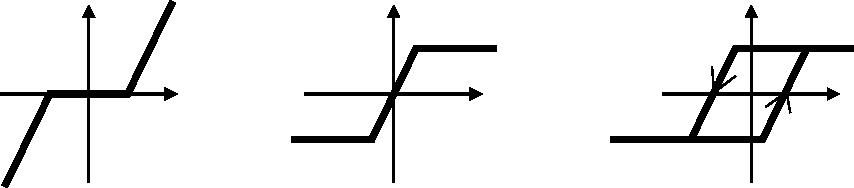
\includegraphics[width=0.4\linewidth]{img/non_lineaire}}
  \item Il est possible de procéder à une linéarisation autour d'un point donné (étude locale), cela n'est valable que pour des durées faibles.
\end{itemize}\vspace{-0.5cm}
\end{rem}
}}


{\frame{
\frametitle{Systèmes invariants}

Un système est invariant si la relation entre l'entrée et la sortie est indépendante du temps.


\begin{center}
\tikzstyle{int}=[draw, minimum size=2em]
\tikzstyle{init} = [pin edge={to-,thin,black}]

\begin{tikzpicture}[node distance=2.5cm,auto,>=latex']
    \node [int] (a) {Système invariant};
    \node (b) [left of=a,node distance=2cm, coordinate] {a};
    \node [coordinate] (end) [right of=a, node distance=2cm]{};
    \path[->] (b) edge node {$E(t)$} (a);
    \path[->] (a) edge node {$S(t)$} (end);
\end{tikzpicture}
\end{center}\vspace{-0.5cm}

\begin{itemize}
 \item A tout instant $t$, la relation entre les entrées et les sorties s'écrit : $\forall t, S(t)=f(E(t))$ où $f$ est une fonction indépendante de $t$.
\end{itemize}

\begin{rem}\vspace{-0.5cm}
\begin{itemize}
 \item Si $x(t)$ a pour réponse $y(t)$, alors $x(t+Dt)$ pour réponse $y(t+Dt)$,
 \item Les paramètres du système sont indépendants du temps.
\end{itemize}
\end{rem}

\begin{defi}
\textbf{Systèmes dynamiques Continus Linéaires Invariants ou SCLI} : Un Système dynamique est Linéaire Continu et Invariant s'il vérifie simultanément ces propriétés. On utilise, en général, l'abréviation \textbf{S.L.C.I.}. Dans la suite, nous n'étudierons que ce type de système.
\end{defi}
}}

\section{Modélisation de SLCI}

 \ifdef{\public}{\begin{frame}
\frametitle{Table des matières}
\tableofcontents[currentsection]
\end{frame}}{}

{\frame{
\frametitle{Systèmes Linéaires Continus et Invariants}

Un Système Linéaire Continu et Invariant (S.C.L.I.) peut être représentée par une équation différentielle linéaire à coefficients constants.


\begin{center}
\tikzstyle{int}=[draw, minimum size=2em]
\tikzstyle{init} = [pin edge={to-,thin,black}]

\begin{tikzpicture}[node distance=2.5cm,auto,>=latex']
    \node [int] (a) {S.L.C.I.};
    \node (b) [left of=a,node distance=2cm, coordinate] {a};
    \node [coordinate] (end) [right of=a, node distance=2cm]{};
    \path[->] (b) edge node {$E(t)$} (a);
    \path[->] (a) edge node {$S(t)$} (end);
\end{tikzpicture}
\end{center}

\begin{itemize}
 \item A tout instant t, la relation entre l'entrée $E(t)$ et la sortie $S(t)$ s'écrit : \\
\end{itemize}

\begin{center}
$\sum\limits_{i=0}^m a_i.e^{(i)}(t)=\sum\limits_{j=0}^n b_j.s^{(j)}(t)$
\end{center}
avec $n\geq m$ dans les systèmes physiques.

\begin{itemize}
 \item  $e^{(i)}$ est la dérivée i\textsuperscript{ème} de la fonction $e$ par rapport à une variable réelle temps $t$,
 \item $a_i$ est le coefficient de rang $i$ constant indépendant du temps,
 \item $s^{(j)}$ est la dérivée j\textsuperscript{ème} de la fonction  $s$ par rapport à une variable réelle temps $t$,
 \item $b_j$ est le coefficient de rang $j$ constant indépendant du temps.
\end{itemize}
}}

{\frame{
\frametitle{Exemple électrique}

\begin{center}
 \includegraphics[width=0.7\linewidth]{img/schema_elec}
\end{center}
\begin{itemize}
 \item A t=0, le contact K se ferme, et le condensateur se charge. Pour prévoir le comportement de ce système, il faut établir une équation différentielle qui traduit son comportement.
\end{itemize}

\reponse[4]

}}

{\frame{
\frametitle{Exemple mécanique}

\begin{center}
 \includegraphics[width=0.3\linewidth]{img/schema_meca}
\end{center}
\begin{itemize}
 \item Soit le système mécanique composé d'une masse en mouvement $m$, attachée à un bâti par ressort de raideur $k$ et un amortisseur de coefficient de viscosité $b$,
 \item A un instant $t=0$, un effort extérieur horizontal noté $e(t)$ est appliqué instantanément. Pour prévoir le comportement de ce système, il faut établir une équation différentielle qui traduit son comportement.
 \item On désigne par $s(t)$ l'écart de position par rapport à la position d'équilibre.
\end{itemize}

\reponse[3]

}}

{\frame{
\frametitle{Exemple hydraulique}

\begin{center}
 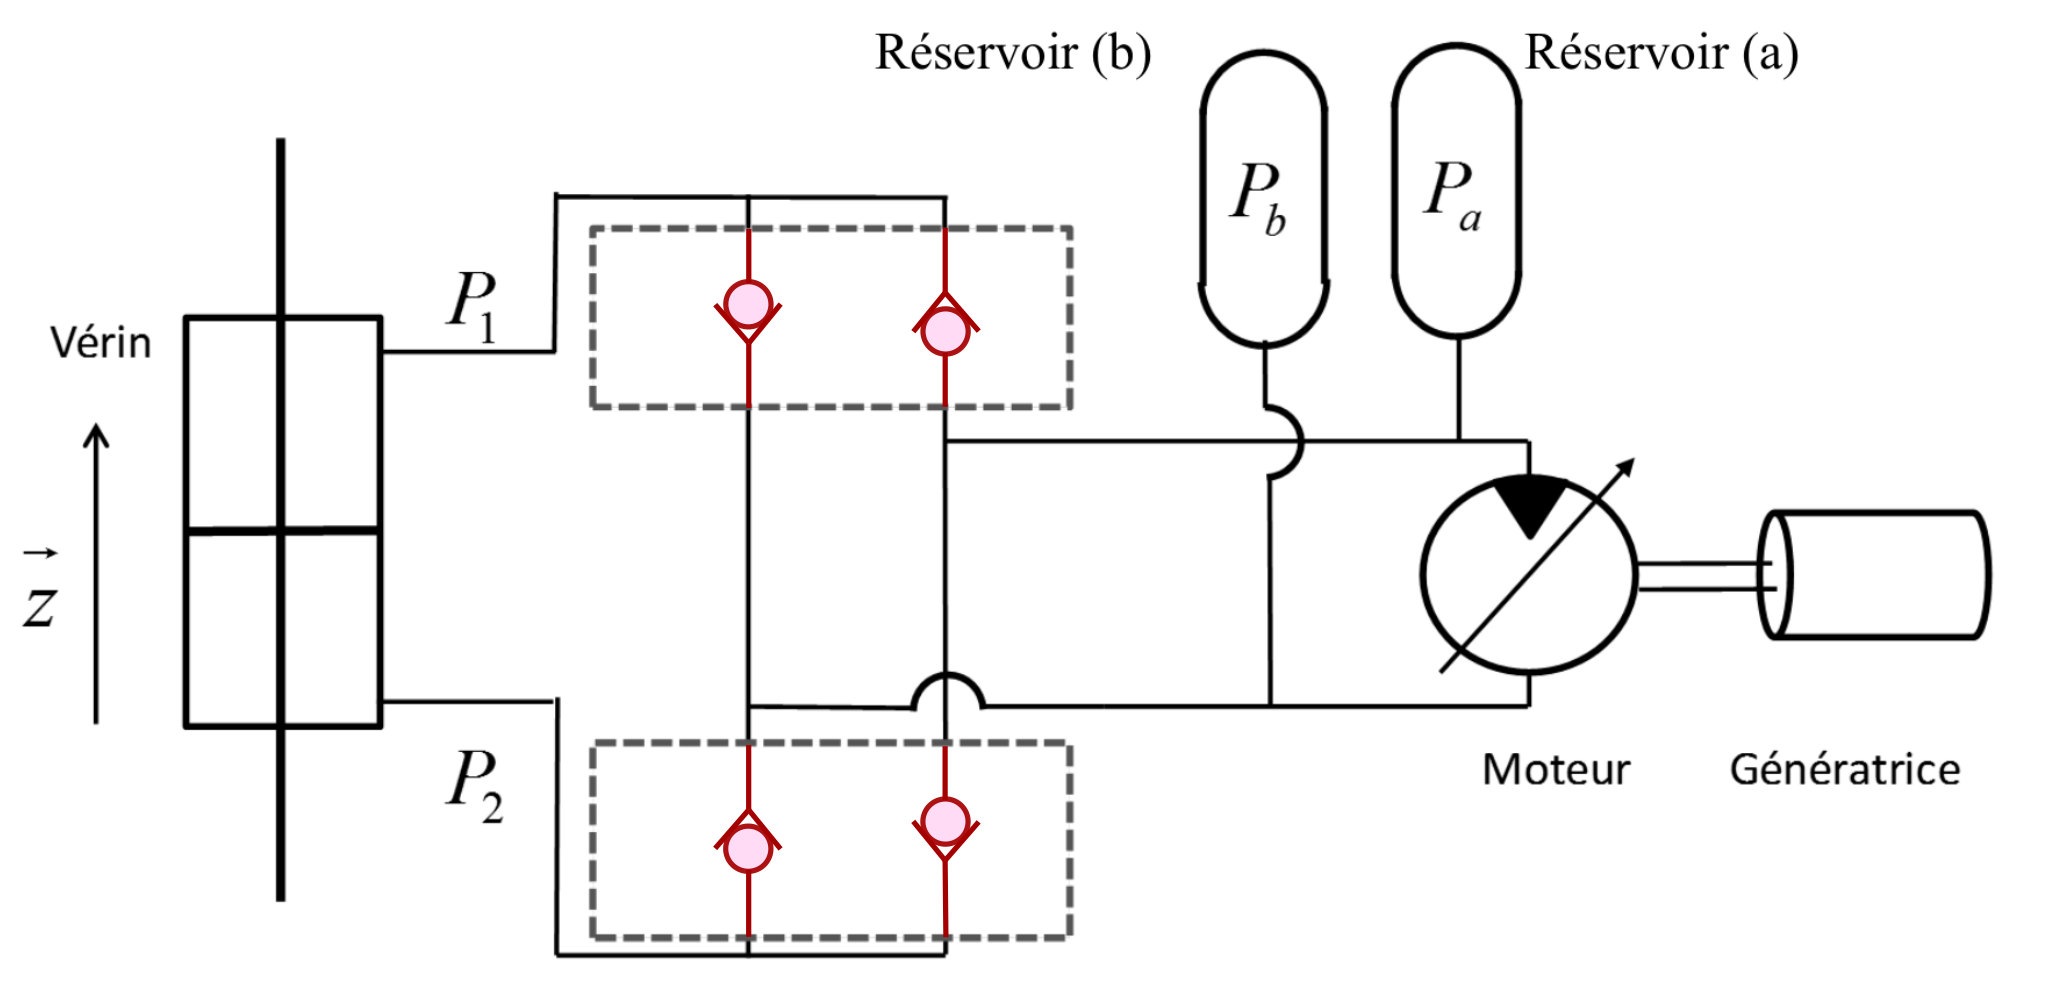
\includegraphics[width=0.2\linewidth]{img/hydraulique}
\end{center}
\begin{itemize}
 \item Soit le système hydraulique composé d'un réservoir de section $S$. On note $s(t)$ la hauteur de liquide dans le réservoir. Elle est alimentée par un conduit dont le débit volumique instantané est noté $e(t)$. Le débit volumique instantané de fuite du réservoir est noté $q(t)$.
 \item A un instant $t=0$, le débit instantané prend un valeur finie non nulle $e(t)$.
\end{itemize}

\reponse[3]
}}

\section{Transformations de Laplace}

 \ifdef{\public}{\begin{frame}
\frametitle{Table des matières}
\tableofcontents[currentsection]
\end{frame}}{}

{\frame{
\frametitle{Transformations de Laplace}

Soit $f(t)$ une fonction de la variable réelle $t$ définie sur $\mathbb{R}$ et supposée nulle pour tout $t<0$  (\og fonction causale\fg). La \textbf{transformée de Laplace} de la fonction $f(t)$ est la fonction complexe $F(p)$ de la variable complexe $p$, définie par l'intégrale, (si elle converge...):

\begin{center}
$F(p)= \int_{0}^{+\infty} f(t).e^{-pt}.dt$
\end{center}

\begin{rem}
 \begin{itemize}
 \item Notation: $F(p)=L[f(t)]$,
 \item Pour $t<0$ la fonction $f(t)$ est nulle, les valeurs prises par $f(t)$ pour $t<0$ n'interviennent pas,
 \item Pour cela, multiplier la fonction $f(t)$ quelconque par la fonction \og échelon \fg notée $u(t)$,
  \begin{itemize}
   \item $u(t)=0$ pour $t<0$,
   \item $u(t)=1$ pour $t>0$.
  \end{itemize}
 \item Si $f(t)=cos(wt)$, calculer la transformée de Laplace de $cos(wt).u(t)$. 
 \end{itemize}
\end{rem}
}}

{\frame{
\frametitle{Propriétés de la transformation de Laplace}

\textbf{Unicité} 

A $f(t)$ correspond une et une seule fonction $F(p)$ et inversement.

\textbf{Linéarité (ou superposition)}

$L[a.f(t)+b.g(t)]=a.L[f(t)]+b.L[g(t)]$.

\textbf{Théorème de la dérivée première}

$L[f'(t)]=p.F(p)-f(0+)$, $f(0+)$ représente la valeur à l'origine de la fonction $f$ (C.I.).

\textbf{Théorème de la dérivée seconde} 

$L\left[\dfrac{d^2 f(t)}{dt^2}\right]=p^2.F(p)-p.f(0+)-f'(0+)$.

\textbf{Théorème de l'intégrale première} 

$L\left[\int_{0}^{+\infty} f(t)dt\right]=\dfrac{1}{p}.F(p)$.	
}}

{\frame{
\frametitle{Propriétés de la transformation de Laplace}

\textbf{Théorème du retard}

$L\left[f(t-\tau)\right]=e^{-\tau.p}.F(p)$

\textbf{Théorème de la valeur initiale}

$\lim\limits_{t \rightarrow 0} f(t)=\lim\limits_{p \rightarrow +\infty} p.F(p)$ \footnotemark[1].

\textbf{Théorème de la valeur finale}

$\lim\limits_{t \rightarrow +\infty} f(t)=\lim\limits_{p \rightarrow 0} p.F(p)$ \footnotemark[1].

[1] Ces résultats n'ont de sens que si les limites existent, elles sont liées à des conditions sur la fonction $F(p)$.
}}

{\frame{
\frametitle{Exemples de transformées}

\begin{minipage}{0.7\linewidth}
\textbf{Fonction impulsion, ou \og pic de DIRAC \fg}

$e(t)>0$ pour $t=0$ et $\int_{-\infty}^{+\infty} e(t).dt=1$

Transformation de Laplace : \\
En remarquant que $e^{-pt}.\delta(t)=0$ pour $t\in[\epsilon,+\infty]$ et $e^{-pt}.\delta(t)=\delta(t)$ pour $t\in[0,+\epsilon]$. 
\begin{center}
	$L[\delta(t)]=1$
\end{center}
\end{minipage}\hfill
\begin{minipage}{0.25\linewidth}
\includegraphics[width=0.95\linewidth]{img/dirac}
\end{minipage}

\vfill

\begin{minipage}{0.7\linewidth}
\textbf{Fonction échelon}

La fonction échelon est définie par : $u(t)=1$ pour $t\geq 0$, $u(t)=0$ pour $t<0$.

Transformation de Laplace : \\
$L[u(t)]=\int_{0}^{+\infty}1.e^{-pt}.dt=\left[-\dfrac{1}{p}e^{-pt}\right]_0^{+\infty}=-\dfrac{1}{p}.e^{-p.\infty}+\dfrac{1}{p}$

\begin{center}
$L[u(t)]=\dfrac{1}{p}$
\end{center}
\end{minipage}\hfill
\begin{minipage}{0.25\linewidth}
\includegraphics[width=0.95\linewidth]{img/echelon}
\end{minipage}
}}

{\frame{
\frametitle{Exemples de transformées}

\textbf{Fonction rampe} Définie par $f(t)=t.u(t)$, $L[t.u(t)]=\int_{0}^{+\infty}t.e^{-pt}.dt$

\begin{minipage}{0.7\linewidth}

Transformation de Laplace (Intégration par parties): \\ 
\begin{flushleft}
$L[t.u(t)]=\left[-t.\dfrac{1}{p}.e^{-pt}\right]_0^{+\infty}-\int_0^{\infty}-\dfrac{1}{p}.e^{-pt}.dt=-\left[\dfrac{1}{p^2}.e^{-pt}\right]_0^{+\infty}$
\end{flushleft}

\begin{center}
	$L[t.u(t)]=\dfrac{1}{p^2}$
\end{center}
\end{minipage}\hfill
\begin{minipage}{0.25\linewidth}
\includegraphics[width=0.95\linewidth]{img/rampe}
\end{minipage}

\vfill

\textbf{Fonction décroissance exponentielle} $f(t)=e^{-at}.u(t)$

\begin{minipage}{0.7\linewidth}

Transformation de Laplace : \\
\begin{flushleft}
$L[e^{-at}.u(t)]=\int_{0}^{+\infty}e^{-pt}.e^{-at}.dt=-\dfrac{1}{p+a}\left[-e^{-(p+a).t}\right]_0^{+\infty}$
\end{flushleft}

\begin{center}
$L[e^{-at}.u(t)]=\dfrac{1}{p+a}$
\end{center}
\end{minipage}\hfill
\begin{minipage}{0.25\linewidth}
\includegraphics[width=0.95\linewidth]{img/expo}
\end{minipage}
}}

{\frame{
\frametitle{Transformée inverse de Laplace}

La fonction $f(t)$ dont $F(p)$ est la transformée, est appelée \textbf{fonction originale} de $F(p)$.

$F(p)=L[f(t)] \Leftrightarrow f(t)=L^{-1}[F(p)]$

La résolution du problème dans le \og domaine symbolique \fg fournit une équation en \og p \fg. Il faut identifier cette équation à des transformées (fonctions de \og p \fg) figurant dans le tableau, et dont on connaît donc les transformées inverses. L'équation dans le \og domaine temporel \fg ainsi obtenue est la solution recherchée.

\begin{rem}
 \begin{itemize}
 \item La transformée inverse d'une \textbf{somme} de fonctions dans le domaine de Laplace \textbf{est égale} à la somme des transformées inverses.
 $L^{-1}\left[F_1(p)+F_2(p)+...+F_n(p)\right]=L^{-1}\left[F_1(p)\right]+L^{-1}\left[F_2(p)\right]+...+L^{-1}\left[F_n(p)\right]$
 \item La transformée inverse d'un \textbf{produit} de fonctions dans le domaine de Laplace \textbf{n'est pas égale} au produit des transformées inverses. (Il faut utiliser une décomposition en éléments simples pour transformer le produit en somme.)
 \st{$L^{-1}\left[F_1(p)\times F_2(p)\times ...\times F_n(p)\right]=L^{-1}\left[F_1(p)\right]\times L^{-1}\left[F_2(p)\right]\times ...\times L^{-1}\left[F_n(p)\right]$}
 \end{itemize}
\end{rem}
}}

{\frame{
\frametitle{Résolution d'un cas simple}

Soit à résoudre l'équation différentielle donnant la vitesse d'un corps en chute libre dans le vide : $\dfrac{dv(t)}{dt}=g$. Les conditions initiales sont nulles, c'est à dire que $V_0=0$.

\begin{enumerate}
 \item Le mouvement ne débute qu'à $t=0$ (l'attraction terrestre ne s'applique qu'a partir de $t=0$). Ainsi $\dfrac{dv(t)}{dt}=g.u(t)$,
 \item Passage dans le domaine de Laplace: $L\left[\dfrac{dv(t)}{dt}\right]=p.V(p)-v(0+)=p.V(p)$ et à la transformée connue de $u(t)$: $L[u(t)]=\dfrac{1}{p}$,
 \item Cela donne l'équation symbolique suivante: $p.V(p)=g.\dfrac{1}{p}$
 \item La résolution se passe dans le domaine symbolique: $V(p)=g.\dfrac{1}{p^2}$
 \item Calcul de la transformation inverse en sachant que $\dfrac{1}{p^2}$ est la transformée de $t.u(t)$. 
\end{enumerate}

$v(t)=g.t.u(t)$ est la solution de l'équation dans le domaine temporel.
}}

{\frame{
\frametitle{Représentation par fonction de transfert}

Pour caractériser le S.C.L.I., il n'est pas nécessaire de déterminer la \textbf{Réponse} $s(t)$ du système à une \textbf{Consigne} $e(t)$. En se plaçant dans le cas particulier où les Conditions Initiales sont nulles et en appliquant la méthode de Laplace, on obtient la relation :

\begin{center}
$\left(t\rightarrow \sum\limits_{i=0}^m a_i.e^{(i)}(t)=\sum\limits_{j=0}^n b_j.s^{(j)}(t)\right)\rightarrow 
\left(p\rightarrow \left(\sum\limits_{i=0}^m a_i.p^i\right).E(p)=\left(\sum\limits_{j=0}^n b_j.p^j\right)S(p)\right)$
\end{center}

\vspace{-0.5cm}

D'où: $\dfrac{S(p)}{E(p)}=H(p)=\dfrac{\sum\limits_{i=0}^m a_i.p^i}{\sum\limits_{j=0}^n b_j.p^j}$ qui peut s'écrire $S(p)=H(p).E(p)$ avec des C.I. nulles.

Le rapport $H(p)$ est indépendant de l'entrée de Consigne $e(t)$ et la Réponse de sortie $s(t)$. Cette fraction rationnelle est appelée la \textbf{Fonction de Transfert} du S.C.L.I.

\begin{minipage}{0.35\linewidth}
Notation, si $z_i$ est le i\textsuperscript{ème} zéro du numérateur de $H(p)$ et $p_i$ le i\textsuperscript{ème} pôle de $H(p)$ (zéro du polynôme du dénominateur):
\end{minipage}\hfill
\begin{minipage}{0.5\linewidth}
$H(p)=\dfrac{k_1.\prod\limits_{i=1}^m (z_i-p)}{k_2.\prod\limits_{j=1}^n (p_j-p)}=\dfrac{K}{p^{\alpha}}.\dfrac{\prod\limits_{i=1}^m \left(1-\dfrac{p}{z_i}\right)}{\prod\limits_{j=1}^n \left(1-\dfrac{p}{p_j}\right)}$
\end{minipage}
}}

{\frame{
\frametitle{Représentation par fonction de transfert}

La forme canonique de la Fonction de Transfert $H(p)$ est l'écriture suivante de $H(p)$:

\begin{center}
$H(p)=\dfrac{K}{p^{\alpha}}.\dfrac{\prod\limits_{i=1}^m \left(1-\dfrac{p}{z_i}\right)}{\prod\limits_{j=1}^n \left(1-\dfrac{p}{p_j}\right)}=\dfrac{K}{p^{\alpha}}.\dfrac{N^*(p)}{D^*(p)}$, avec $\dfrac{N^*(0)}{D^*(0)}=1$
\end{center}

\begin{itemize}
 \item \textbf{Classe} : La Classe de la Fonction de Transfert $H(p)$ est le nombre $\alpha$ de Pôles nuls,
 \item \textbf{Gain} : Le Gain de la Fonction de Transfert $H(p)$ est le coefficient $K$. Lorsque $\alpha=0$, ce Gain s'appelle le Gain Statique de la Fonction de Transfert,
 \item \textbf{Ordre} : L'Ordre de la fonction de Transfert est le degré du dénominateur de la Fonction de Transfert,
 \item Le polynôme au dénominateur est aussi appelé polynôme caractéristique du système.
\end{itemize}
}}

{\frame{
\frametitle{Pôles et stabilité d'un S.C.L.I.}

Si on représente les Pôles (complexes à priori) de la fonction de transfert dans le plan représentant la Partie Imaginaire $Im(p)$ du Pôle $p$ en fonction de sa partie Réelle $Re(p)$, on peut avoir une idée de la réponse à une entrée impulsionnelle.

\begin{center}
 \includegraphics[width=0.5\linewidth]{img/poles_stabilite}
\end{center}

\begin{rem}
\vspace{-0.5cm}
\begin{itemize}
 \item Si la partie Réelle du Pôle est \textbf{positive} le système est \textbf{instable},
 \item Si la partie Réelle du Pôle est \textbf{nulle}, le système \textbf{oscille} sans s'amortir.
\end{itemize}
\end{rem}
}}

\section{Réponses temporelles}

 \ifdef{\public}{\begin{frame}
\frametitle{Table des matières}
\tableofcontents[currentsection]
\end{frame}}{}

{\frame{
\frametitle{Réponse temporelle d'un système intégrateur (Classe 1 et ordre 1)}

\begin{itemize}
 \item A tout instant $t$, la relation entre l'entrée $e(t)$ et la sortie $s(t)$ s'écrit : $\dot{s}(t)=K.e(t)$.
 \item Il se traduit par la fonction de transfert suivante : $H(p)=\dfrac{K}{p}$, avec le \textbf{gain} K en $\dfrac{[s(t)]}{[e(t)].s}$.
 \item Si on cherche la \textbf{réponse indicielle}, $e(t)=u(t)$ qui a pour transformée de Laplace : $E(p)=\dfrac{1}{p}$
\end{itemize}

\begin{minipage}{0.5\linewidth}
La réponse du système est (CI nulles): \\
$S(p)=\dfrac{K}{p}.E(p)=\dfrac{K}{p}.\dfrac{1}{p}=\dfrac{K}{p^2}$ .

Cette fonction a pour Transformée Inverse : \\
$s(t)=K.t$, $t\in \left[0,+\infty\right[$.

Réponse indicielle pour un $K=1$ en $\dfrac{[s(t)]}{[e(t)].s}$.
\end{minipage}\hfill
\begin{minipage}{0.45\linewidth}
\begin{center}
 \includegraphics[width=0.9\linewidth]{img/integrateur}
\end{center}
\end{minipage}
}}

{\frame{
\frametitle{Réponse temporelle (Système du 1\textsuperscript{er} ordre)}

A tout instant $t$, la relation entre l'entrée $e(t)$ et la sortie $s(t)$ s'écrit : $s(t)+\tau.\dot{s}(t)=K.e(t)$.

\begin{resultat}
\vspace{-0.3cm}
Il se traduit par la fonction de transfert suivante : $H(p)=\dfrac{K}{1+\tau.p}$.\vspace{-0.3cm}
\end{resultat}

Avec des \textbf{conditions initiales nulles}, c'est-à-dire , la réponse du système est : 

$S(p)=H(p).E(p)=\dfrac{K}{1+\tau.p}.E(p)=\dfrac{K}{1+\tau.p}.\dfrac{1}{p}=\dfrac{K}{p(1+\tau.p)}=K\left[\dfrac{A}{p}+\dfrac{B}{1+\tau.p}\right]$

\begin{itemize}
 \item Si $p\rightarrow 0 \Rightarrow K=K.\left[A+B.0\right] \Rightarrow A=1$,
 \item Si $p\rightarrow +\infty \Rightarrow 0=K.\left[A.\tau+B\right] \Rightarrow B=-\tau$.
\end{itemize}

\begin{resultat}\vspace{-0.3cm}
Donc: \hspace{1cm} $S(p)=K.\left[\dfrac{1}{p}-\dfrac{\tau}{1+\tau.p}\right] \rightarrow s(t)=K.\left(1-e^{\dfrac{-t}{\tau}}\right), t\in\left[0,+\infty\right[$\vspace{-0.3cm}
\end{resultat}

Pente à l'origine : $\dfrac{K}{\tau}$, la tangente à l'origine est : $y=\dfrac{K}{\tau}.t$
}}

{\frame{
\frametitle{Réponse temporelle (Système du 1\textsuperscript{er} ordre)}

\begin{center}
	\includegraphics[width=0.7\linewidth]{img/temp_ordre1}
\end{center}
}}

{\frame{
\frametitle{Réponse temporelle (Système du 1\textsuperscript{er} ordre)}

\begin{prop}
La tangente à la courbe à un instant $t_0$ donné intercepte l'asymptote à l'infini un instant $t_0+\tau$.
\end{prop}

\begin{minipage}{0.5\linewidth}
L'équation de la tangente à la courbe à un instant $\boldsymbol{t_0}$ est :
$y=\dot{s}(t_0)(t-t_0)+s(t_0)$

$\Rightarrow y=\dfrac{K}{\tau}.e^{\dfrac{-t_0}{\tau}}(t-t_0)+K.\left(1-e^{\dfrac{-t_0}{\tau}}\right)$

Interception de l'asymptote à l'infini pour: $y=K$. \\
Donc : $K=\dfrac{K}{\tau}.e^{\dfrac{-t_0}{\tau}}(t-t_0)+K.\left(1-e^{\dfrac{-t_0}{\tau}}\right)$

\begin{resultat}
Les deux droites s'interceptent au temps: $t=t_0+\tau$
\end{resultat}

\end{minipage}\hfill
\begin{minipage}{0.45\linewidth}
 \includegraphics[width=0.9\linewidth]{img/pente_origine}
\end{minipage}
}}

{\frame{
\frametitle{Réponse temporelle (Système du 2\textsuperscript{ème} ordre)}

A tout instant t, la relation entre $e(t)$ et $s(t)$ s'écrit : $\omega_0^2.s(t)+2.\xi.\omega_0.\dot{s}(t)+\ddot{s}(t)=K.\omega_0^2.e(t)$

\begin{resultat}\vspace{-0.3cm}
Il se traduit par la fonction de transfert suivante : $H(p)=\dfrac{K}{1+\dfrac{2.\xi}{\omega_0}.p+\left(\dfrac{p}{\omega_0}\right)^2}$\vspace{-0.3cm}
\end{resultat}

Réponse (CI nulles): 
$S(p)=H(p).E(p)=\dfrac{K}{1+\dfrac{2.\xi}{\omega_0}.p+\left(\dfrac{p}{\omega_0}\right)^2}.\dfrac{1}{p}=\dfrac{K.\omega_0^2}{\left(p^2+2.\xi.\omega_0.p+\omega_0^2\right).p}$

\begin{rem}\vspace{-0.5cm}
\begin{itemize}
 \item $\boldsymbol{K}$ est le \textbf{gain statique} (en $\dfrac{[s(t)]}{[e(t)]}$),
 \item $\boldsymbol{\xi}$ est le \textbf{facteur d'amortissement} (adimensionnel). Si $\xi$ est grand devant 1, le système est très dissipatif,
 \item $\omega_0$ est la \textbf{pulsation propre} (en radian par seconde $rd.s^{-1}$). Si $\omega_0$ est grand devant $1rd.s^{-1}$, le système est rapide.
 \end{itemize}\vspace{-0.3cm}
\end{rem}
}}

{\frame{
\frametitle{Réponse temporelle (Système du 2\textsuperscript{ème} ordre)}

Il faut tout d'abord rechercher les pôles de la fonction de transfert. Pour cela, on résout l'équation caractéristique : \\
$p^2+2.\xi.\omega_0.p+\omega_0^2=0 \Rightarrow \Delta=(2.\xi.\omega_0)^2-4.\omega_0^2=4.\xi^2.\omega_0^2-4.\omega_0^2=4.\omega_0^2.\left(\xi^2-1\right)$

\begin{itemize}
 \item Cas 1: $\Delta>0 \Leftrightarrow 4.\omega_0^2.\left(\xi^2-1\right)>0 \Leftrightarrow \xi^2 > 1  \Leftrightarrow \xi > 1$,
 \item Cas 2: $\Delta=0 \Leftrightarrow 4.\omega_0^2.\left(\xi^2-1\right)=0 \Leftrightarrow \xi^2 = 1  \Leftrightarrow \xi = 1$,
 \item Cas 3: $\Delta<0 \Leftrightarrow 4.\omega_0^2.\left(\xi^2-1\right)<0 \Leftrightarrow \xi^2 < 1  \Leftrightarrow \xi < 1$,
\end{itemize}

}}

{\frame{
\frametitle{Réponse temporelle (Système du 2\textsuperscript{ème} ordre) $\xi > 1$}

$H(p)$ admet deux pôles réels strictement négatifs $p_1$ et $p_2$ car leur somme $p_1+p_2=-2.\xi.\omega_0<0$ et leur produit $p_1.p_2=\omega_0^2$. Il est donc inutile de les calculer:

\begin{minipage}{0.49\linewidth}
$p_1=-\omega_0.\left(\xi+\sqrt{\xi^2-1}\right)$, si $T_1=-\dfrac{1}{p_1}$ \\
$\Rightarrow \dfrac{1}{T_1}=\omega_0.\left(\xi+\sqrt{\xi^2-1}\right)$
\end{minipage}\hfill
\begin{minipage}{0.49\linewidth}
$p_2=-\omega_0.\left(\xi-\sqrt{\xi^2-1}\right)$, si $T_2=-\dfrac{1}{p_2}$ \\
$\Rightarrow \dfrac{1}{T_2}=\omega_0.\left(\xi-\sqrt{\xi^2-1}\right)$
\end{minipage}

~\

\begin{resultat}
La réponse temporelle est alors: \\
$s(t)=K.\left[1-\dfrac{T_1}{T_1-T_2}.e^{-\dfrac{t}{T_1}}+\dfrac{T_2}{T_1-T_2}.e^{-\dfrac{t}{T_2}}\right]$, $t\in \left[0,+\infty\right[$.
\end{resultat}

}}

{\frame{
\frametitle{Réponse temporelle (Système du 2\textsuperscript{ème} ordre) $\xi > 1$}

$s(t)=K.\left[1-\dfrac{e^{-\omega_0.\xi.t}}{2.\sqrt{\xi^2-1}}.\left[-\left(\xi-\sqrt{\xi^2-1}\right).e^{-\omega_0.\sqrt{\xi^2-1}.t}+\left(\xi+\sqrt{\xi^2-1}\right).e^{\omega_0.\sqrt{\xi^2-1}.t}\right]\right]$

\begin{center}
 \includegraphics[width=0.7\linewidth]{img/ordre2_1}
\end{center}

}}

{\frame{
\frametitle{Réponse temporelle (Système du 2\textsuperscript{ème} ordre) $\xi = 1$}

Dans ce cas, H(p) admet pôle réel double et strictement négatif $p=-\omega_0$.

~\

\begin{resultat}
La réponse temporelle est alors: \\
$s(t)=K.\left[1-\left(1+\omega_0.t\right).e^{-\omega_0.t}\right]$, $t\in \left[0,+\infty\right[$.
\end{resultat}

}}

{\frame{
\frametitle{Réponse temporelle (Système du 2\textsuperscript{ème} ordre) $\xi < 1$}

$H(p)$ admet deux pôles complexes conjugués à partie réelle strictement négative $p_1$ et $\overline{p_1}$ car leur somme $p_1+\overline{p_1}=2.Re(p_1)=-2.\xi.\omega_0<0$

~\

\begin{resultat}
La réponse temporelle est alors: \\
$s(t)=K.\left[1-\dfrac{e^{-\omega_0.\xi.t}}{\sqrt{1-\xi^2}}.cos\left[\left(\omega_0.\sqrt{1-\xi^2}\right).t-arctan\left(\dfrac{\xi}{\sqrt{1-\xi^2}}\right)\right]\right]$, $t\in \left[0,+\infty\right[$.
\end{resultat}

}}

{\frame{
\frametitle{Réponse temporelle (Système du 2\textsuperscript{ème} ordre) $\xi < 1$}

\begin{center}
 \includegraphics[width=0.6\linewidth]{img/ordre2_2}
\end{center}

 \begin{itemize}
 \item \textbf{Pseudo oscillations} dont la \textbf{pseudo-période} $T_p$ est telle que :
  $\left[\omega_0.\sqrt{1-\xi^2}\right].T_p=2.\pi \Rightarrow T_p=\dfrac{2.\pi}{\omega_0.\sqrt{1-\xi^2}}$
 \item Maximum autour de la demi pseudo-période : $T_{max}=\dfrac{T_p}{2}$ 
 \end{itemize}
}}

{\frame{
\frametitle{Réponse temporelle (Système du 2\textsuperscript{ème} ordre) $\xi < 1$}

\begin{minipage}{0.7\linewidth}
Pour caractériser la précision du système insuffisamment amorti pendant la phase transitoire, on détermine le dépassement exprimé en \% qui est donné par la relation :

~\

$D\%=100.\dfrac{S_{max}-s(+\infty)}{s(+\infty)} \Rightarrow D\%=100.\dfrac{S(T_{max})-K}{K}$

~\

\begin{resultat}
$D\%=100.e^{-\xi.\dfrac{\pi}{\sqrt{1-\xi^2}}}$
\end{resultat}
\end{minipage}\hfill
\begin{minipage}{0.25\linewidth}
\includegraphics[width=0.8\linewidth]{img/ordre2_32}
\end{minipage}

Tous ces tracés peuvent être réalisés avec le fichier python à télécharger sur mon compte GitHub dans le dossier du cours S02-C01 \href{https://github.com/Costadoat/Sciences-Ingenieur/raw/master/S02\%20Systèmes\%20Linéaires\%20Continus\%20Invariants/C01\%20Présentation\%20des\%20SLCI/02-C01.py}{ici}.
}}

{\frame{
\frametitle{Réponse temporelle (Système du 2\textsuperscript{ème} ordre) $\xi < 1$}

Pour déterminer le \textbf{temps de réponse à n\%}, il faut déterminer l'instant $t_{R,n\%}$ à partir duquel la Réponse $s(t)$ reste dans une bande de plus ou moins $n\%$ de la valeur finale stable $S(+\infty)$ moins la valeur initiale $s(0)$ soit:

\begin{defi}
Définition de réponse à $n\%$: \\
$|s(t)-s(+\infty)|\leq n\%.\left(s(+\infty)-s(0)\right)$
\end{defi}

Calcul à partir des équations des courbes enveloppes des oscillations afin d'approximer le résultat :

$|s(t_{R,n\%})-s(+\infty)| \simeq \left|K.\left(1\pm \dfrac{e^{-\xi.\omega_0.t_{R,n\%}}}{\sqrt{1-\xi^2}}\right)-K\right|= n\%.\left(s(+\infty)-s(0)\right)=n\%.\left(K-0\right)=n\%.K$

\begin{resultat}
Temps de réponse à $5\%$ (valable pour $\xi<0.7$): \\
$t_{R,5\%}=\dfrac{1}{\xi.\omega_0}.ln(20)$
\end{resultat}
}}

{\frame{
\frametitle{Réponse temporelle (Système du 2\textsuperscript{ème} ordre)}

Comparaison des résultats obtenus pour les différentes valeurs de $\xi$.

\begin{rem}
\begin{itemize}
 \item Si $\xi > 1$, $\searrow$ $\xi \Rightarrow$ (à pulsation propre $\omega_0$ constante) $\nearrow$ rapidité, $\searrow$ $t_R$,
 \item Si $\xi < 1$, $\searrow$ $\xi \Rightarrow$ (apparition de pseudo-oscillations) $\searrow$ rapidité, $\nearrow$ $t_R$,
\end{itemize}
\end{rem}

\begin{minipage}{0.45\linewidth}
 \includegraphics[width=1\linewidth]{img/ordre2_3}
\end{minipage}\hfill
\begin{minipage}{0.45\linewidth}
 \includegraphics[width=0.8\linewidth]{img/ordre2_4}
\end{minipage}
}}

{\frame{
\frametitle{La modélisation des S.L.C.I.}

\begin{savoir}
Vous devez être capables :
\begin{itemize}
 \item De modéliser un S.L.C.I.
\end{itemize}
\end{savoir}

\begin{prob}
Il est nécessaire d'utiliser d'autres formes de représentation d'un mécanisme.
\begin{itemize}
 \item \textit{Problème: Comment représenter la structure d'un SLCI ?}
 \item \textbf{Perspectives}: Trouver un modèle de description d'un S.L.C.I. afin de gérer les systèmes complexes.
\end{itemize}
\end{prob}
}}


\end{document}

